\documentclass[../main.tex]{subfiles}
\begin{document}
	
	\chapter{Introdução}
	Para iniciar os estudos de Álgebra Linear, é interessante apresentar, inicialmente, conceitos básicos para visualizar e estruturar o conhecimento. Nesse sentido, entender vetores na perspectiva geométrica, ou seja, no plano ($\mathbb{R}^2$) ou no espaço ($\mathbb{R}^3$), é mais intuitivo em um primeiro contato. Nos próximos capítulos, em especial no capítulo 3, a definição de vetores será ampliada para outros espaços vetoriais, com um maior nível de abstração.
	
	\section{Álgebra Vetorial}
		Embora iniciemos com Álgebra Vetorial e não Geometria Analítica, é interessante começar com um ponto de vista mais geométrico, para criar intuição.
		\begin{definicao}
			\azul{Vetores (geometricamente)} são objetos matemáticos que possuem módulo, direção e sentido.
			
			Usualmente, um vetor é representado por segmentos de retas orientados equipolentes, ou seja, que apresentam mesmo tamanho, direção e sentido.
			\begin{center}
				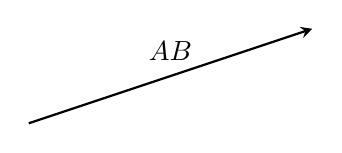
\begin{tikzpicture}[scale=1.2, >=stealth]
					\draw[thick] [->] (0,0) -- (3,1) node[midway, above=2pt] {$\vv{AB}$};
				\end{tikzpicture}
			\end{center}
		\end{definicao}
		Note que, pela definição, um vetor não possui "origem fixa" e pode ser representado por diferentes segmentos de reta orientados.
		\begin{definicao}
			Sejam $U$ e $V$ vetores representados por $\vv{AB}$ e $\vv{BC}$, respectivamente. A \azul{soma de vetores} $U+V$ é definida como o vetor representado pelo segmento de reta orientado $\vv{AC}$  
			\begin{center}
				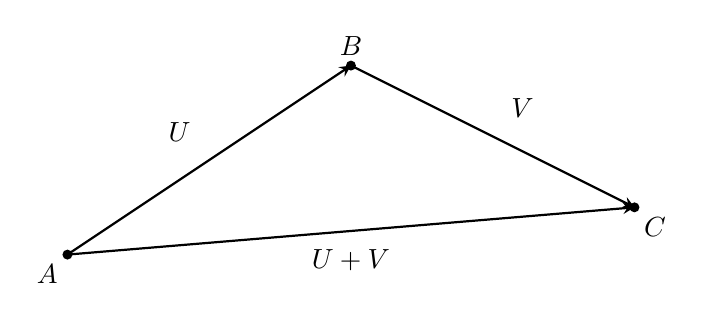
\begin{tikzpicture}[scale=1.2, >=stealth]
					% Pontos
					\coordinate (A) at (0,0);
					\coordinate (B) at (3,2);
					\coordinate (C) at (6,0.5);
					
					% Lados com setas
					\draw[thick, ->] (A) -- (B) node[midway, above left=3pt] {$U$};
					\draw[thick, ->] (B) -- (C) node[midway, above right=3pt] {$V$};
					\draw[thick, ->] (A) -- (C) node[midway, below=3pt] {$U+V$};
					
					% Pontos marcados
					\fill (A) circle (1.5pt) node[below left] {$A$};
					\fill (B) circle (1.5pt) node[above] {$B$};
					\fill (C) circle (1.5pt) node[below right] {$C$};
				\end{tikzpicture}
			\end{center}
		\end{definicao}
		\begin{proposicao}
			Sejam $V$, $W$ e $U$ vetores.
			A soma de vetores segue as seguintes propriedades:
			\begin{enumerate}[label=\roman*)]
				\item $V+W=W+V$ (comutatividade)
				\item $V+(W+U)=(V+W)+U$ (associatividade)
				\item $\exists \text{ vetor }\bar{0}\text{, tal que }  V+\bar{0}=V$ (existência do elemento neutro/vetor nulo)
			\end{enumerate}
		\end{proposicao}
		Abaixo seguem ilustrações das propriedades \textit{i)} e \textit{ii)}.
		\begin{figure}[h!]
			\centering
			\begin{minipage}{0.45\textwidth}
				\centering
				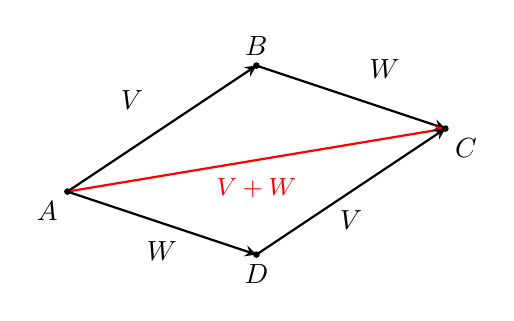
\begin{tikzpicture}[scale=0.8, >=stealth]
					% Pontos
					\coordinate (A) at (0,0);
					\coordinate (B) at (3,2);
					\coordinate (C) at (6,1);
					\coordinate (D) at (3,-1);
					
					% Lados com setas
					\draw[thick, ->] (A) -- (B) node[midway, above left=3pt] {$V$};
					\draw[thick, ->] (B) -- (C) node[midway, above right=3pt] {$W$};
					\draw[thick, ->, red] (A) -- (C) node[midway, below=3pt] {\small $V+W$};
					\draw[thick, ->] (A) -- (D) node[midway, below=3pt] {$W$};
					\draw[thick, ->] (D) -- (C) node[midway, below=3pt] {$V$};
					
					% Pontos marcados
					\fill (A) circle (1.5pt) node[below left] {$A$};
					\fill (B) circle (1.5pt) node[above] {$B$};
					\fill (C) circle (1.5pt) node[below right] {$C$};
					\fill (D) circle (1.5pt) node[below] {$D$};
				\end{tikzpicture}
			\end{minipage}
			\hfill
			\begin{minipage}{0.45\textwidth}
				\centering
				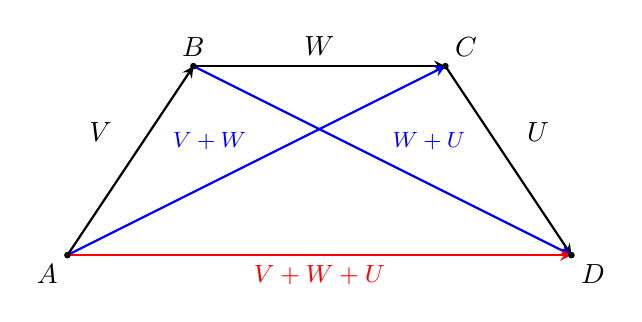
\begin{tikzpicture}[scale=0.8, >=stealth]
					% Pontos
					\coordinate (A) at (0,0);
					\coordinate (B) at (2,3);
					\coordinate (C) at (6,3);
					\coordinate (D) at (8,0);
					
					% Lados com setas
					\draw[thick, ->] (A) -- (B) node[midway, above left=3pt] {$V$};
					\draw[thick, ->] (B) -- (C) node[midway, above] {$W$};
					\draw[thick, ->] (C) -- (D) node[midway, above right=3pt] {$U$};
					\draw[thick, ->, blue] (A) -- (C) node[midway, above left] {\footnotesize $V+W$};
					\draw[thick, ->, blue] (B) -- (D) node[midway, above right] {\footnotesize $W+U$};
					\draw[thick, ->, red] (A) -- (D) node[midway, below] {\small $V+W+U$};
					
					% Pontos marcados
					\fill (A) circle (1.5pt) node[below left] {$A$};
					\fill (B) circle (1.5pt) node[above] {$B$};
					\fill (C) circle (1.5pt) node[above right] {$C$};
					\fill (D) circle (1.5pt) node[below right] {$D$};
				\end{tikzpicture}
			\end{minipage}
		\end{figure}
		\begin{definicao}
			Seja $V$ um vetor. Seu \azul{simétrico}, denotado por $-V$, é o vetor tal que
			\[
			V+(-V)=\bar{0}
			\]
		\end{definicao}
		\begin{definicao}
			Sejam $V$ e $W$ vetores. A \azul{diferença $W$ menos $V$} é definida como
			\[
			W-V=W+(-V)
			\]
		\end{definicao}
		\begin{definicao}
			Sejam $V\neq \bar{0}$ um vetor e $\alpha\neq 0$ um escalar (ou seja, um número real). A \azul{multiplicação do vetor $V$ por um escalar $\alpha$}, denotada por $\alpha V$, é definida pelo vetor tal que:
			\begin{enumerate}[label=\roman*)]
				\item seu módulo é $|\alpha||V|$, onde $|V|$ é o módulo de $V$;
				\item a direção é a mesma de $V$;
				\item tem sentido de $V$ se $\alpha>0$, e sentido de $-V$ se $\alpha<0$.
			\end{enumerate}
			Caso $V=\bar{0}$ ou $\alpha=0$, $\alpha V=\bar{0}$
		\end{definicao}
		Note, portanto, que, para um vetor qualquer $W$ ser paralelo (ou seja, ter a mesma direção que) a outro vetor $V$, baste que exista um $\alpha\in \mathbb{R}$ tal que $W=\alpha V$. 
		\begin{definicao}
			Seja $V$ um vetor. As \azul{componentes de V} são cada elemento das coordenadas que representam o ponto final com relação à origem do sistema de coordenadas escolhido.
			
			Se $V$ está no plano (\azul{$\mathbb{R}^2$} ou \azul{espaço euclidiano bidimensional}), então suas coordenadas são uma trupla de dois números reais, denotadas usualmente por $(v_1, v_2)$.
			
			Se $V$ está no espaço (\azul{$\mathbb{R}^3$} ou \azul{espaço euclidiano tridimensional}), então suas coordenadas são uma tupla de três números reais, denotadas usualmente por $(v_1, v_2, v_3)$.
			
			Se $V$ está em "dimensões maiores" (\azul{$\mathbb{R}^n$} ou \azul{espaço euclidiano n-dimensional}), então suas coordenadas são uma tupla de $n$ números reais, denotadas usualmente por $(v_1, \dots, v_n)$.
		\end{definicao}
		Na Figura \ref{fig:vetores-R2-R3}, seguem ilustrações de como coordenadas funcionam no plano e no espaço.
		\begin{figure}[h]
			\centering
			
			% --- subfigura R^2 ---
			\begin{subfigure}[t]{0.48\textwidth}
				\centering
				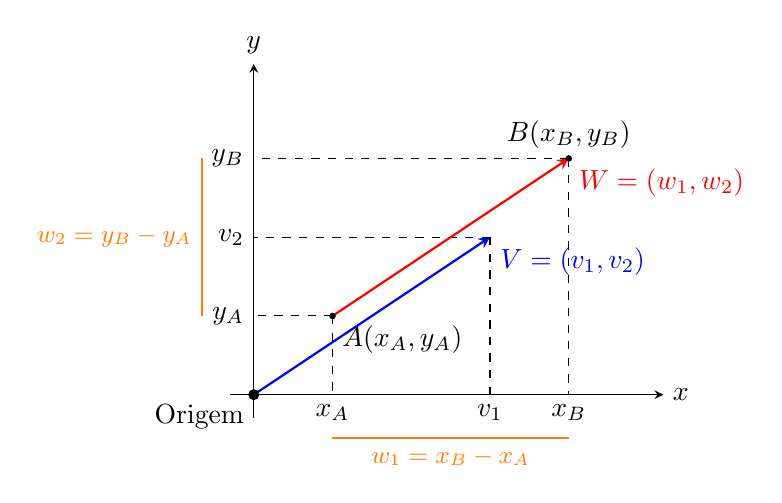
\begin{tikzpicture}[>=stealth,scale=1.0] % pode ajustar a escala se quiser
					% Eixos
					\draw[->] (-0.3,0) -- (5.2,0) node[right] {$x$};
					\draw[->] (0,-0.3) -- (0,4.2) node[above] {$y$};
					
					\coordinate (O) at (0,0);
					\coordinate (P) at (3,2);   % ponto de v
					\coordinate (A) at (1,1);   % ponto inicial de w
					\coordinate (B) at (4,3);   % ponto final de w
					
					% Vetor na origem
					\draw[->,thick,blue] (O) -- (P)
					node[below right] {$V=(v_1,v_2)$};
					
					% Projeções de v
					\draw[dashed] (P) -- (3,0) node[below] {$v_1$};
					\draw[dashed] (P) -- (0,2) node[left] {$v_2$};
					
					% Vetor deslocado
					\draw[->,thick,red] (A) -- (B)
					node[below right] {$W=(w_1,w_2)$};
					
					% Pontos A e B e orgigem
					\fill (A) circle (1.2pt) node[below right] {$A(x_A,y_A)$};
					\fill (B) circle (1.2pt) node[above] {$B(x_B,y_B)$};
					\fill (O) circle (2pt) node[below left] {\text{Origem}};
					
					% Projeções para mostrar diferenças
					\draw[dashed] (A) -- (1,0) node[below] {$x_A$};
					\draw[dashed] (B) -- (4,0) node[below] {$x_B$};
					\draw[dashed] (A) -- (0,1) node[left] {$y_A$};
					\draw[dashed] (B) -- (0,3) node[left] {$y_B$};
					
					% Segmentos representando as diferenças
					\draw[thick,orange,yshift=-10pt]
					(1,-0.2) -- node[below] {\small $w_1 = x_B - x_A$} (4,-0.2);
					
					\draw[thick,orange,xshift=-13pt]
					(-0.2,1) -- node[left] {\small $w_2 = y_B - y_A$} (-0.2,3);
				\end{tikzpicture}
				\caption{Representação no $\mathbb{R}^2$.}
			\end{subfigure}
			\hfill
			% --- subfigura R^3 ---
			\begin{subfigure}[t]{0.48\textwidth}
				\centering
				\tdplotsetmaincoords{70}{120}
				\begin{tikzpicture}[scale=1.6,tdplot_main_coords,>=stealth]
					% Eixos
					\draw[->] (0,0,0) -- (3,0,0) node[below right] {$x$};
					\draw[->] (0,0,0) -- (0,3,0) node[left] {$y$};
					\draw[->] (0,0,0) -- (0,0,3) node[above] {$z$};
					
					% Vetor na origem
					\coordinate (V) at (1,1.4,3);
					\draw[->,thick,blue] (0,0,0) -- (V)
					node[below right] {$V=(v_1,v_2,v_3)$};
					\fill (0,0,0) circle (1.5pt) node[above left] {\text{Origem}};
					\fill (V) circle (1.5pt) node[above left] {};
					
					% Projeções de v
					\coordinate (Vxy) at (1,1.4,0);
					\coordinate (Vx)  at (1,0,0);
					\coordinate (Vy)  at (0,1.4,0);
					\draw[dashed] (V) -- (Vxy);
					\draw[dashed] (Vxy) -- (Vx) node[above left] {$v_1$};
					\draw[dashed] (Vxy) -- (Vy) node[above right] {$v_2$};
					\draw[dashed] (V) -- (0,0,3) node[left] {$v_3$};
					\draw[dashed] (0,0,0) -- (Vxy);
				\end{tikzpicture}
				\caption{Representação no $\mathbb{R}^3$.}
			\end{subfigure}
			
			\caption{Componentes de vetores em $\mathbb{R}^2$ e $\mathbb{R}^3$.}
			\label{fig:vetores-R2-R3}
		\end{figure}
		
		Perceba que, para verificar as componentes de um vetor qualquer $W$ representado por um segmento $\vv{AB}$, basta subtrair as suas coordenadas, de modo que:
		\[
		W = \vv{AB}\Rightarrow
		\begin{cases}
			w_1 = x_B - x_A\\
			w_2 = y_B - y_A
		\end{cases}\Rightarrow
		W = (x_B - x_A,\, y_B - y_A)
		\]
		Para o $\mathbb{R}^3$, a subtração ocorre da mesma forma.
		
		Com isso, note que as operações ficam muito mais fáceis, sem depender sempre do apelo geométrico. Assim, podemos buscar uma nova forma de fazer as operações básicas entre vetores (soma e multiplicação por escalar):
		\needspace{5\baselineskip}
		\begin{proposicao}
			Sejam $V, W\in \mathbb{R}^2$ e $\alpha\in \mathbb{R}$. Então,
			\begin{enumerate}[label = \roman*)]
				\item $V+W = (v_1+w_1,\, v_2+w_2)$
				\item $\alpha V = (\alpha v_1,\, \alpha v_2)$
			\end{enumerate} 
		\end{proposicao}
		Abaixo temos uma ilustração disso.
		\begin{figure}[h]
			\centering
			
			%----------------- (a) Soma de vetores -----------------
			\begin{subfigure}[t]{0.48\textwidth}
				\centering
				\begin{tikzpicture}[>=stealth,scale=1.2]
					
					% Eixos
					\draw[->] (-0.3,0) -- (4.5,0) node[right] {$x$};
					\draw[->] (0,-0.3) -- (0,3.5) node[above] {$y$};
					
					\coordinate (O) at (0,0);
					\coordinate (V) at (2,1.0);   % V = (v1,v2)
					\coordinate (W) at (1.2,1.6); % W = (w1,w2)
					\coordinate (S) at ($(V)+(W)$); % V+W
					
					% Vetores V e W na origem
					\draw[->,thick,blue] (W) -- (S)
					node[below right] {$ V$};
					\draw[->,thick,red]  (O) -- (W)
					node[above left] {$W$};
					
					% Vetor soma
					\draw[->,thick,green!60!black] (O) -- (S)
					node[above right] {$ V+ W$};
					
					% Projeções
					\draw[dashed] (W) -- (1.2, 0) node[below] {$w_1$};
					\draw[dashed] (W) -- (0, 1.6) node[left] {$w_2$};
					\draw[dashed] (S) -- (3.2, 0) node[below] {$w_1+v_1$};
					\draw[dashed] (S) -- (0, 2.6) node[left] {$w_2+v_2$};
					
					% Segmentos representando as diferenças
					\draw[thick,orange,yshift=-10pt]
					(1.2,-0.2) -- node[below] {\small $v_2$} (3.2,-0.2);
					
					\draw[thick,orange,xshift=-13pt]
					(-0.2,1.6) -- node[left] {\small $v_1$} (-0.2,2.4);
					
				\end{tikzpicture}
				\caption{Soma de vetores: $ V+ W=(v_1+w_1,\;v_2+w_2)$.}
			\end{subfigure}
			\hfill
			%----------------- (b) Multiplicação escalar -----------------
			\begin{subfigure}[t]{0.48\textwidth}
				\centering
				\begin{tikzpicture}[>=stealth,scale=1.2]
					
					% Eixos
					\draw[->] (-0.3,0) -- (4.5,0) node[right] {$x$};
					\draw[->] (0,-0.3) -- (0,3.5) node[above] {$y$};
					
					\coordinate (O) at (0,0);
					\coordinate (V) at (1.8,1.1);     % V
					\def\alpha{2}                      % escolha de alpha > 1
					\coordinate (AV) at ({\alpha*1.8},{\alpha*1.1}); % alpha V
					
					% vetor V
					\draw[->,thick,blue] (0,0) -- (1.8,1.1)
					node[below right] {$V = (v_1,v_2)$};
					
					% vetor 2V um pouco acima, para não ficar em cima de V
					\draw[->,thick,red] (0,0.1) -- (3.6,2.3)
					node[above right] {$2V = (2v_1,2v_2)$};
					
				\end{tikzpicture}
				\caption{Multiplicação escalar: $\alpha V=(\alpha v_1,\alpha v_2)$.}
			\end{subfigure}
			
			\caption{Ilustração da soma de vetores e multiplicação escalar em $\mathbb{R}^2$.}
		\end{figure}
		
		Para o $\mathbb{R}^3$, essas operações ocorrem da mesma forma. Generalizando para qualquer dimensão ($\mathbb{R}^n$), temos:
		
		\begin{proposicao}
			Sejam $V, W\in \mathbb{R}^n$ e $\alpha\in \mathbb{R}$. Então,
			\begin{enumerate}[label = \roman*)]
				\item $V+W = (v_1+w_1,\dots, \, v_n+w_n)$
				\item $\alpha V = (\alpha v_1,\dots ,\, \alpha v_n)$
			\end{enumerate} 
		\end{proposicao}
		E se quisermos fazer ambas as operações ao mesmo tempo? Então teremos uma combinação linear!
		\begin{definicao}
			Sejam $V_1, \dots, V_k \in \mathbb{R}^n$ vetores e $\alpha_1,\dots, \alpha_k \in \mathbb{R}$ escalares. Seja $W$ um vetor tal que
			\[
			W = \alpha_1 V_1 + \dots + \alpha_k V_k 
			\]
			Então, $W$ é \azul{combinação linear} de $V_1, \dots, V_k$.
		\end{definicao}
		Abordaremos melhor esse conceito em tópicos mais a frente, como em sistemas lineares.
		
		A partir da definição de coordenadas e da soma/multiplicação de vetores por meio delas, podemos provar as seguintes propriedades:
		\begin{teorema}
			Sejam $U$, $V$ e $W$ vetores e $\alpha$ e $\beta$ escalares. Então,
			\begin{multicols}{2}
				\begin{enumerate}[label=\roman*)]
					\item $U+V=V+U$;
					\item $(U+V)+W=U+(V+W)$;
					\item $U+\bar{0}=U$;
					\item $U+(-U)=\bar{0}$;
					\item $\alpha(\beta U)=(\alpha \beta)U$;
					\item $\alpha(U+V)=\alpha U+\alpha V$;
					\item $(\alpha+\beta)U=\alpha U+\beta U$;
					\item $1U=U$.
				\end{enumerate}
			\end{multicols}
			\label{teo:vetores8axiomas}
		\end{teorema}
		
		Outra ideia muito importante é saber o módulo do vetor a partir de seus componentes. Para isso, vamos definir o que chamamos de norma euclidiana.
		\begin{definicao}
			Seja $V\in \mathbb{R}^n$. O seu comprimento, também chamado de \azul{norma de $V$} e denotado por $\|V\|$, é dado por
			\[
			\|V\|=\sqrt{v_1^2 +\dots + v_n^2}
			\]
		\end{definicao}
		
		\begin{exemplo}
			Para um vetor  $V\in \mathbb{R}^2$, temos que
			\[
			\|V\| = \sqrt{v_1^2+v_2^2}
			\]
		\end{exemplo}
		\begin{figure}[h]
			\centering
			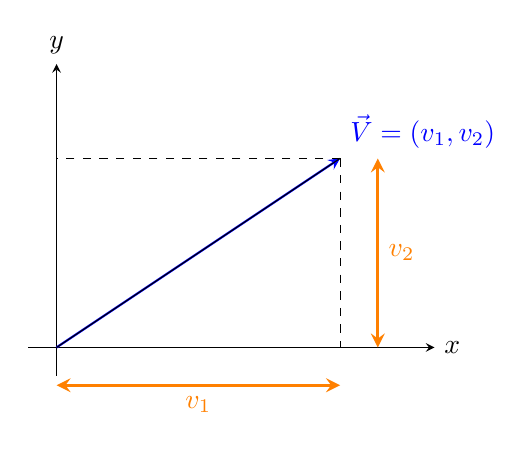
\begin{tikzpicture}[>=stealth,scale=1.2]
				
				% Eixos
				\draw[->] (-0.3,0) -- (4,0) node[right] {$x$};
				\draw[->] (0,-0.3) -- (0,3) node[above] {$y$};
				
				% Vetor V
				\coordinate (O) at (0,0);
				\coordinate (V) at (3,2);   % V = (v1,v2)
				\coordinate (Vx) at (3,0);
				\coordinate (Vy) at (0,2);
				
				\draw[->,thick,blue] (O) -- (V)
				node[above right] {$\vec V=(v_1,v_2)$};
				
				% Projeções para formar o triângulo retângulo
				\draw[dashed] (V) -- (Vx);
				\draw[dashed] (V) -- (Vy);
				
				% Catetos rotulados v1 e v2
				\draw[<->,orange, very thick]
				(0,-0.4) -- node[below] {$v_1$} (3, -0.4);
				\draw[<->,orange,very thick]
				(3.4,0) -- node[right] {$v_2$} (3.4, 2);
				
				% Marcação do ângulo reto
				\tkzMarkRightAngle(V,Vx,O)
				
				% Rótulo da norma na hipotenusa
				\draw (O) -- (V)
				node[midway,above left,yshift=4pt]
				{};
				
			\end{tikzpicture}
			\caption{Norma de um vetor $\vec V$ em $\mathbb{R}^2$.}
		\end{figure}
		Essa forma de calcular a norma está ligada ao cálculo do tamanho de vetores no $\mathbb{R}^2$ e no $\mathbb{R}^3$, utilizando o Teorema de Pitágoras.
		
		A partir dessa definição de norma, podemos definir outro conceito fundamental: o produto escalar. Este produto pega dois vetores e devolve um escalar (número real), que vai indicar o "nível de alinhamento entre eles".
		
		\begin{definicao}
			Sejam $V,\, W\in \mathbb{R}^n$, onde $n\in \{2,3\}$. O \azul{produto escalar} (também conhecido como \azul{produto interno}) entre esses vetores, denotado por $V\cdot W$, é dado por
			\[
			V\cdot W = \begin{cases}
				0\text{, se $V=\bar{0}$ ou $W=\bar{0}$}\\
				\|V\|\|W\|\cos(\theta)\text{, caso contrário.}
			\end{cases}
			\]
			onde $\theta$ é o ângulo no intervalo $[0,\pi]$ entre eles. 
		\end{definicao}
		Note, no entanto, que o ângulo entre dois vetores só é bem definido para vetores em $\mathbb{R}^2$ ou $\mathbb{R}^3$. Para resolver esse problema, podemos encontrar uma definição equivalente para o produto escalar e depois generalizá-la para dimensões maiores.
		\begin{proposicao}
			Sejam $V$ e $W$ vetores. Então, seu produto escalar é dado por
			\[
			V\cdot W = \begin{cases}
				v_1w_1+v_2w_2\text{, se $V,W \in \mathbb{R}^2$}\\
					
					v_1 w_1 +v_2 w_2 + v_3 w_3\text{, se $V, W \in \mathbb{R}^3$.}
			\end{cases}
			\]
		\end{proposicao}
		A partir disso, podemos definir o produto escalar da seguinte forma generalizada.
		\begin{definicao}
			Sejam $V, W\in \mathbb{R}^n$. O produto escalar entre esses vetores, denotado por $V\cdot W$, é dado por
			\[
			V\cdot W = v_1 w_1+\dots + v_n w_n
			\]
		\end{definicao}
		Com essa definição, podemos facilmente provar as seguintes propriedades (que futuramente definirão de forma ainda mais abrangente o produto interno).
		\begin{proposicao}
			Sejam $U,\, V,\, W\in \mathbb{R}^n$ e $\alpha \in \mathbb{R}$. Então:
			\begin{enumerate}[label=\roman*)]
				\item $U\cdot V=V\cdot U$;
				\item $U\cdot (V+W)=U\cdot V+U\cdot W$;
				\item $\alpha(U\cdot V)=(\alpha U)\cdot V = U\cdot (\alpha V)$;
				\item $V\cdot V=\|V\|^2\geq 0$
				
				$V\cdot V=\|V\|^2=0 \Leftrightarrow V = \bar{0}$.
			\end{enumerate}
		\end{proposicao}
		As ideias de norma e produto escalar são essenciais e possuem interpretação geométrica. O produto escalar, por exemplo, mostra a relação entre os tamanhos e "alinhamento" (ângulo) entre dois vetores. Isso é muito bem visualizado ao tentarmos entender projeções de um vetor sobre outro: a projeção ortogonal.
		
		\begin{definicao}
			Sejam $V$ e $W$ vetores. A \azul{projeção ortogonal de $V$ sobre $W$}, denotada por $\text{proj}_W V$ é o vetor tal que
			\begin{itemize}
				\item $\text{proj}_W V \parallelsum W$ (a projeção e $W$ têm a mesma direção);
				\item $V-\text{proj}_W V \perp W$ (a diferença de $V$ com a projeção é perpendicular a $W$).
			\end{itemize}
		\end{definicao}
		Abaixo segue uma ilustração da projeção ortogonal.
		\begin{figure}[h]
			\centering
			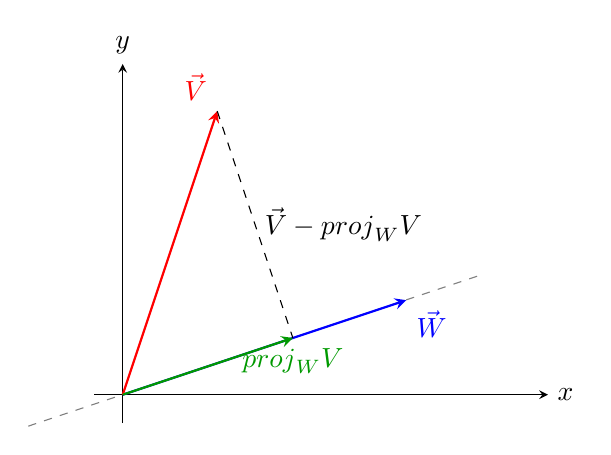
\begin{tikzpicture}[>=stealth,scale=1.2]
				
				% Eixos
				\draw[->] (-0.3,0) -- (4.5,0) node[right] {$x$};
				\draw[->] (0,-0.3) -- (0,3.5) node[above] {$y$};
				
				% Pontos e vetores
				\coordinate (O) at (0,0);
				\coordinate (W) at (3,1);    % direção de W
				\coordinate (V) at (1,3);    % vetor V
				\coordinate (P) at (1.8,0.6);% proj_W V  (ponto na reta de W)
				
				% Reta gerada por W (para ver bem a projeção)
				\draw[dashed,gray] (-1,-1/3) -- (3.8,1.27);
				
				% Vetor W
				\draw[->,thick,blue] (O) -- (W)
				node[below right] {$\vec W$};
				
				% Vetor V
				\draw[->,thick,red] (O) -- (V)
				node[above left] {$\vec V$};
				
				% Projeção de V sobre W
				\draw[->,thick,green!60!black] (O) -- (P)
				node[below] {$\operatorname{proj}_W V$};
				
				% Componente ortogonal V - proj_W V
				\draw[dashed] (V) -- (P)
				node[midway,right] {$\vec V - \operatorname{proj}_W V$};
				
				% Marcação do ângulo reto
				\tkzMarkRightAngle(W,P,V)
				
			\end{tikzpicture}
			\caption{Projeção ortogonal de $\vec V$ sobre $\vec W$.}
		\end{figure}
		
		A partir dessa definição, podemos provar o seguinte teorema.
		\begin{teorema}
			Seja $W\neq \bar{0}$ um vetor. Então,
			\[
			\text{proj}_W V = \bigg(\frac{V\cdot W}{\|W\|^2}\bigg)W
			\]
		\end{teorema}
		Além do produto escalar, existem outros dois produtos essenciais da Álgebra Vetorial. Enquanto o produto escalar trabalha com "alinhamentos" e projeções, o produto vetorial e misto representam, respectivamente, área e volume.
		\begin{definicao}
			Sejam $V,\, W\in \mathbb{R}^3$. O \azul{produto vetorial} (também conhecido como \azul{produto externo}) entre esses vetores, denotado por $V\times W$, é dado por
			\[
			V\times W = \begin{cases}
				\bar{0}\text{, se $V=\bar{0}$ ou $W=\bar{0}$}\\
				U\text{, caso contrário.}
			\end{cases}
			\]
			onde $U$ é definido como o vetor tal que:
			\begin{enumerate}[label=\roman*)]
				\item $\|U\|=\|V\|\|W\|\sin(\theta)$;
				\item $U\perp V$ e $U\perp W$;
				\item o sentido é dado pela regra da mão direita.
			\end{enumerate}
		\end{definicao}
		A regra da mão direita estabelece que os dedos giram de $V$ para $W$ e o polegar aponta na direção de $U$ (movimento representado na Figura \ref{fig:maodireita}). Perceba que, caso invertamos a ordem de $W$ para $V$, a direção também é alterada.
		
		Utilizando as componentes dos vetores, podemos obter as coordenadas do seu produto vetorial de uma forma mais simples.
		\begin{proposicao}
			Sejam $V,\, W\in \mathbb{R}^3$. Então,
			\[
			V\times W = \bigg( \det \begin{bmatrix}
				v_2 & v_3\\
				w_2 & w_3
			\end{bmatrix}, -\det \begin{bmatrix}
				v_1 & v_3\\
				w_1 & w_3
			\end{bmatrix}, \det \begin{bmatrix}
				v_1 & v_2\\
				w_1 & w_2
			\end{bmatrix}\bigg)
			\]
			Ou, utilizando um abuso de notação, temos
			\[
			V\times W = \det \begin{bmatrix}
				\vec i & \vec j & \vec k\\
				v_1 & v_2 & v_3\\
				w_1 & w_2 & w_3
			\end{bmatrix}
			\]
			onde $\vec i=(1, 0, 0)$, $\vec j=(0,1,0)$ e $\vec k=(0,0,1)$ são os \azul{vetores canônicos}.
		\end{proposicao}
		\begin{figure}[h]
			\centering
			% vista 3D
			\tdplotsetmaincoords{70}{120}
			\begin{tikzpicture}[tdplot_main_coords,scale=2,>=stealth]
				
				\coordinate (O) at (0,0,0);
				
				% Vetores a e b no plano xy
				\draw[->,thick] (O) -- (2,0,0)
				node[below right] {$V$};
				\draw[->,thick] (O) -- (0,2,0)
				node[below left] {$W$};
				
				% Produto vetorial a x b (polegar)
				\draw[->,very thick,blue] (O) -- (0,0,2)
				node[above] {$V \times W$};
				
				% Arco mostrando o sentido de a para b (sentido dos dedos)
				\draw[->,thick]
				(1.4,0,0) arc[start angle=0,end angle=90,radius=1.4]
				node[midway,below] {$\text{sentido dos dedos}$};
				
			\end{tikzpicture}
			\caption{Regra da mão direita}
			\label{fig:maodireita}
		\end{figure}
		
		Se você não estiver habituado às ideias de matrizes e determinante, não se preocupe. No capítulo 2, apresentaremos formalmente cada um.
		
		Note que, no abuso de notação para representar o produto vetorial, temos que os componentes da matriz são ora vetores, ora números reais, o que indica uma matriz inválida. A ideia dessa representação é de que, se considerássemos $\vec i$, $\vec j$ e $\vec k$ números reais e fizéssemos a conta de tal determinante, e a multiplicação entre reais fosse igual à multipliação por escalar, teríamos o equivalente à primeira forma do produto vetorial, apresentada imediatamente antes. Em suma, essa segunda representação é, na verdade, um "macete" para decorar o produto vetorial.
		
		A partir dessas definições equivalentes do produto vetorial, podemos demonstrar as seguintes propriedades.
		\begin{proposicao}
			Sejam $U,\, V,\, W\in \mathbb{R}^3$ e $\alpha \in \mathbb{R}$. Então:
			\begin{enumerate}[label=\roman*)]
				\item $V\times W=-(W\times V)$;
				\item $V\times W=\bar{0}\Leftrightarrow V=\alpha W\text{ ou } W=\alpha V \text{ (ou seja, caso sejam paralelos)}$;
				\item $(V\times W)\cdot V=(V\times W)\cdot W=0$;
				\item $\alpha(V\times W)=(\alpha V)\times W=V\times (\alpha W)$;
				\item $V\times (W+U)=V\times W+V\times U$ e $(V+W)\times U=V\times U+W\times U$.
			\end{enumerate}
		\end{proposicao}
		Já o produto misto é dado pela "mistura" dos dois conceitos apresentados anteriormente.
		\begin{definicao}
			Sejam $V,\, W, \, U \in \mathbb{R}^3$. Então, o \azul{produto misto}, denotado por $[V, W, U]$, é dado por
			\[
			[V, W, U]=(V\times W)\cdot U
			\]
		\end{definicao}
		A partir dos conceitos de produto vetorial e escalar, podemos descrever o misto de uma forma facilitada, bem como ressaltar algumas propriedades interessantes.
		\begin{proposicao}
			Sejam $V,\, W, \, U \in \mathbb{R}^3$. Então, 
			\[
			[V, W, U]=\det \begin{bmatrix}
				v_1 & v_2 & v_3\\
				w_1 & w_2 & w_3\\
				u_1 & u_2 & u_3
			\end{bmatrix}
			\]
		\end{proposicao}
		\begin{proposicao}
			Sejam $V,\, W, \, U\in \mathbb{R}^3$ e $\alpha \in \mathbb{R}$. Então,
			\begin{enumerate}[label=\roman*)]
				\item $[U+Z,V,W]=[U,V,W]+[Z,V,W]$
				
				$[U,V+Z,W]=[U,V,W]+[U,Z,W]$
				
				$[U,V,W+Z]=[U,V,W]+[U,V,Z]$;
				\item $[U,V,W]=-[U,W,V]=-[W,V,U]=-[V,U,W]$;
				\item $[U,V,W]=U\cdot(V\times W)$;
				\item $\alpha[U, V, W]=[\alpha U, V, W]=[U, \alpha V, W]=[U, V, \alpha W]$.
			\end{enumerate}
		\end{proposicao}
		Como dito, anteriormente, os produtos vetorial e misto possuem uma interpretação geométrica interessante. Isso se deve ao fato de que, quando os vetores $V$, $W$ e $U$ são não nulos, temos $\|V\times W\|=\|V\|\|W\|\sin(\theta_1)$ e $|[V,W,U]|=\|V\times W\|\|U\|\cos(\theta_2)$.
		
		Essas definições permitem o entendimento de que a norma do produto vetorial é a área do paralelogramo formado pelos vetores $V$ e $W$, e o módulo do produto misto é o volume do paralelepípedo. Na Figura \ref{fig:areavolume}, temos uma ilustração de como isso ocorre.
		
		\begin{figure}[htb]
			\centering
			
			%---- Subfigura 1 ----
			\begin{subfigure}[b]{0.45\textwidth}
				\centering
				\begin{tikzpicture}[>=stealth,scale=1.2]
					%--- Coordenadas ---
					\coordinate (O) at (0,0);
					\coordinate (V) at (4,0);
					\coordinate (W) at (1.2,3);
					\coordinate (S) at ($(V)+(W)$);
					\coordinate (P) at (1.2,0);
					
					
					%--- Vetores ---
					\draw[thick,->, red] (O) -- (V) node[midway,below] {$V$};
					\draw[thick,->, blue] (O) -- (W) node[midway,left] {$W$};
					\draw[dashed] (V) -- (S);
					\draw[dashed] (W) -- (S);
					
					%--- Projeção (altura) ---
					\draw[dashed] (W) -- node[right] {$h=\|W\|\sin\theta_1$} (P);
					
					%--- Ângulo theta com arco manual ---
					\draw (0.5,0) arc[start angle=0, end angle=68, radius=0.5];
					\node at (0.8,0.25) {$\theta_1$};
				\end{tikzpicture}
				\caption{Área do paralelogramo.}
			\end{subfigure}
			%---- Subfigura 2 ----
			\begin{subfigure}[b]{0.45\textwidth}
				\centering
				\begin{tikzpicture}[
					scale=1.2,
					>=stealth,
					x={(1cm,0cm)},        % eixo x: horizontal
					y={(0.7cm,0.35cm)},   % eixo "pra dentro" (y)
					z={(0cm,1cm)}         % eixo z: vertical
					]
					%--- pontos básicos ---
					\coordinate (O)  at (0,0,0);      % origem
					\coordinate (H)  at (0,0,1.8);    % topo da altura h
					\coordinate (V)  at (2.0,0,0);      % vetor v no "chão"
					\coordinate (U)  at (1.6, 0.3, 1.8);% ponta de u
					\coordinate (W)  at (1.2,0.6,0);  % direção de w (no chão)
					
					% pontos derivados
					\coordinate (VW)   at ($(V)+(W)$);
					\coordinate (UW)   at ($(U)+(W)$);
					\coordinate (UV)   at ($(U)+(V)$);
					\coordinate (UVW)  at ($(U)+(V)+(W)$);
					
					%--- base e paralelepípedo (linhas tracejadas) ---
					% base da frente
					\draw[->,thick, red] (O) -- (V) node[below right] {$V$};
					% base "de trás" (passando por w)
					\draw[dashed] (W) -- (VW);
					% laterais tracejadas
					\draw[dashed] (V)  -- (VW);
					\draw[dashed] (W)  -- (UW);
					\draw[dashed] (V)  -- (UV);
					\draw[dashed] (UW) -- (UVW);
					\draw[dashed] (UV) -- (UVW);
					\draw[dashed] (VW) -- (UVW);
					\draw[dashed] (U) -- (UV);
					\draw[dashed] (U) -- (UW);
					
					%--- altura h ---
					\draw[dashed] (O) -- (H) node[above] {$h=\|U\|\cos \theta_2$};
					\draw[dashed] (H) -- (U);
					\tkzMarkRightAngle(O,H,U)
					
					%--- angulo teta 2 ---
					\draw (0,0,0.3) arc[start angle=90, end angle=46.5, radius=0.4] node[left=5pt] {$\theta_2$};
					
					%--- vetores principais ---
					% w saindo da origem, indo "pra dentro"
					\draw[->,thick,blue] (O) -- (W) node[above left] {$W$};
					
					% u saindo da origem
					\draw[->,thick, green!60!black] (O) -- (U) node[above right] {$U$};
					
				\end{tikzpicture}
				\caption{Volume do paralelepípedo.}
			\end{subfigure}
			
			\caption{Produto vetorial e produto misto.}
			\label{fig:areavolume}
		\end{figure}
		Como sabemos, a área do paralelogramo é dada pelo produto da base com a altura, enquanto o volume do paralelepípedo é dado pelo produto da área da base com a altura. Assim seguem as relações abaixo. \[A_{VW}=bh=\|V\|h=\|V\|\|W\|\sin(\theta_1)=\|V\times W\|\] \[V_{VWU}=A_{VW}b=A_{VW}\|U\|\cos(\theta_2)=\|V\times W\|\|U\|\cos(\theta_2)=|[V,W,U]|\]
		
		Além das suas normas representarem áreas e volumes, os produtos vetorial e misto, assim como o escalar, são indicadores de "alinhamento" entre vetores. A essas características damos o nome de colinearidade e coplanaridade.
		\begin{definicao}
			Dois ou mais vetores são \azul{colineares} se pertencem a uma mesma reta (ou seja, se são paralelos). 
		\end{definicao}
		\begin{definicao}
			Dois ou mais vetores são \azul{coplanares} se pertencem a um mesmo plano.
		\end{definicao}
		Na próxima seção de Geometria Analítica, ficará mais claro o que significa um vetor pertencer a uma reta ou a um plano. De forma intuitiva, isso significa que o segmento de reta orientado que representa um vetor é paralelo à reta ou ao plano em questão.
		
		Como dito anteriormente, ao definir a multiplicação por escalar, implicitamente entendemos as condições de colinearidade no plano.
		
		\begin{proposicao}
			Sejam $V, W\in \mathbb{R}^2$.
			\begin{itemize}
				\item $V$ e $W$ são colineares $\Leftrightarrow \exists \, \alpha \in \mathbb{R}\text{, tal que } V=\alpha W$, ou seja, se um for múltiplo escalar do outro;
				\item $V$ e $W$ são sempre coplanares (pertencem ao $\mathbb{R}^2$).
			\end{itemize}
		\end{proposicao}
		
		Já para o espaço, é possível utilizar as ideias de senos e cossenos que os produtos vetorial e misto trazem, garantindo as propriedades abaixo.
		\begin{proposicao}
			Sejam $V,\, W,\, U\in \mathbb{R}^3$.
			\begin{itemize}
				\item $V$ e $W$ são colineares $\Leftrightarrow V\times W=\bar{0}$;
				\item Dois vetores $V$ e $W$ são sempre coplanares;
				\item $V$, $W$ e $U$ são coplanares $\Leftrightarrow [V, W, U]=0$.
			\end{itemize}
		\end{proposicao}
		
		Outra forma de verificar colinearidade ou coplanaridade, é utilizando a ideia de combinação linear.
		
		\begin{corolario}
			Sejam $U,\, V,\, W\in \mathbb{R}^3$ coplanares não nulos. Então,
			\begin{enumerate}[label=\roman*)]
				\item um dos vetores é combinação linear dos outros dois;
				\item $V$ e $W$ não paralelos $\Rightarrow$ $U$ combinação linear de $V$ e $W$.
			\end{enumerate}
		\end{corolario}
		Um fato interessante é que, a partir do item \textit{i)} do corolário acima, obtemos que a equação $xV+yW+zU=\bar{0}$ tem solução onde $x,y,z\neq 0$. Isso porque, se existem reais $\alpha, \beta$ tais que $\alpha V+\beta W= U$ (definição de combinação linear), então basta tomar $x=\alpha$, $y=\beta$ e $z=-1$.
		
		A observação acima será mais esclarecedora depois de uma boa leitura da seção 2.3.
		
		Com isso, finalizamos a parte de Álgebra Vetorial. Seguem abaixo os exercícios da seção.
		\subsection*{Exercícios}
		
		\begin{enumerate}
			\item (SANTOS, R; 2014; p. 154)
			Verifique se o vetor $U$ é combinação linear de $V$ e $W$:
				\begin{enumerate}[label=\alph*)]
					\item $V=(9,-12,-6)$, $W=(-1,7,1)$, $U=(-4,-6,2)$;
					\item $V=(5,4,-3)$, $W=(2,1,1)$, $U=(-3,-4,1)$.
				\end{enumerate}
			\item (SANTOS, R; 2014; p. 177)
			Demonstre que, se $V$ e $W$ são vetores quaisquer, então:
				\begin{enumerate}[label=\alph*)]
					\item $|V\cdot W|\leq \|V\|\|W\|$;
					\item $\|V+W\|\leq \|V\|+\|W\|$; (Sugestão: mostre que $\|V+W\|^2=(V+W)\cdot (V+W)\leq (\|V\|+\|W\|)^2$, usando o item anterior)
					\item $\big|\|V\|-\|W\| \big|\leq \|V-W\|$. (Sugestão: defina $U=V-W$ e aplique o item anterior a $U$ e $W$)
				\end{enumerate}
			\item (SANTOS, R; 2014; p. 199)
			Calcule o volume do paralelepípedo que tem um dos vértices no ponto $A=(2,1,6)$ e os três vértices adjacentes nos pontos $B=(4,1,3)$, $C=(1,3,2)$ e $D=(1,2,1)$.
			\item (SANTOS, R; 2014; p.201)
			Prove a identidade de Lagrange
			\[
			\|V\times W\|^2=\|V\|^2\|W\|^2-(V\cdot W)^2
			\]
		\end{enumerate}
		
	\section{Geometria Analítica}
		Na Geometria Analítica, estudamos objetos geométricos, como retas e planos, a partir de um sistema de coordenadas. Nesse capítulo, vamos focar nossa atenção principalmente em retas e planos, ampliando a abordagem anterior de vetores. Primeiramente, podemos tentar definir esses objetos do ponto de vista da geometria analítica.
		
		\subsection*{Equações da reta e do plano}
			\begin{definicao}
				Uma \azul{reta} $r \subset \mathbb{R}^2$ (ou $\mathbb{R}^3$) é o conjunto dos pontos $P$
				dados por
				\[
				P = P_0 + t V, \quad t \in \mathbb{R}
				\]
				onde $P_0$ é um ponto fixo e $V\in \mathbb{R}^2$ (ou $\mathbb{R}^3$) é o vetor diretor não nulo.
			\end{definicao}
			\begin{definicao}
				Um \azul{plano} $\pi \subset \mathbb{R}^3$ é o conjunto dos pontos $P$ dados por
				\[
				P = P_0 + t V + s W, \quad t, s \in \mathbb{R},
				\]
				onde $P_0$ é um ponto fixo e $V, W \in \mathbb{R}^3$ são vetores diretores
				não nulos e não colineares.
			\end{definicao}
			\begin{figure}[h]
				\centering
				\begin{subfigure}[t]{0.45\textwidth}
					\centering
					\begin{tikzpicture}[>=stealth,scale=1.2]
						
						% eixos (opcional)
						\draw[->] (-0.5,0) -- (4,0) node[right] {$x$};
						\draw[->] (0,-0.5) -- (0,3) node[above] {$y$};
						
						% ponto P0 e vetor diretor v
						\coordinate (P0) at (1,1);
						\coordinate (Vdir) at (3,2); % P0 + v, só para 	desenhar
						
						% reta r = P0 + t v  (prolongamos para os dois 	lados)
						\draw[dashed] (-0.2,0.4) -- (3.8,2.4);
						
						% vetor diretor v
						\draw[->,thick,blue] (P0) -- (Vdir)
						node[above left] {$V$};
						
						% ponto P na reta (por exemplo t>0)
						\coordinate (P) at (2.2,1.6);
						\fill (P) circle (1pt) node[below right] {$P$};
						
						% ponto P0
						\fill (P0) circle (1.2pt) node[below right] {$P_0$};
						
						% nome da reta
						\node at (3.5,2) {$r$};
						
					\end{tikzpicture}
					\caption{Reta $r \subset \mathbb{R}^2$ dada por $P=P_0+tV$.}
				\end{subfigure}
				\hfill
				\begin{subfigure}[t]{0.45\textwidth}
					\centering
					\tdplotsetmaincoords{70}{135}
					
					\begin{tikzpicture}[tdplot_main_coords,scale=2.2,>=stealth]
						
						% eixos
						\draw[->] (-0.5,0,0) -- (2,0,0) node[above] {$x$};
						\draw[->] (0,-0.5,0) -- (0,2,0) node[above] {$y$};
						\draw[->] (0,0,-0.2) -- (0,0,1.7) node[above] {$z$};
						
						% ponto P0
						\coordinate (P0)  at (0.6,0.5,0.615);
						
						% vetores diretores (pontas dos vetores)
						\coordinate (V)   at (2.0,0.7,1.434);
						\coordinate (W)   at (1.0,1.8,1.228);
						\coordinate (VW)  at (2.4,2.0,2.047);
						
						% retângulo grande do plano (no plano de P0, v e w)
						% A = P0 -0.5 v -0.5 w
						% B = P0 +2   v -0.5 w
						% C = P0 +2   v +2   w
						% D = P0 -0.5 v +2   w
						\coordinate (A) at (-0.3,-0.25,-0.101);
						\coordinate (B) at ( 3.2, 0.25, 1.947);
						\coordinate (C) at ( 4.2, 3.50, 3.479);
						\coordinate (D) at ( 0.7, 3.00, 1.432);
						
						% ponto P no plano (P = P0 + t v + s w, t=1.1, 	s=0.6)
						\coordinate (P) at (2.38,1.5,1.884);
						
						% plano "grande"
						\fill[green!20,opacity=0.15]
						(A) -- (B) -- (C) -- (D) -- cycle;
						
						\draw[thin,green!40!black,opacity=0.5]
						(A) -- (B) -- (C) -- (D) -- cycle;
						
						% vetores diretores
						\draw[->,thick,blue] (P0) -- (V)
						node[pos=0.55,above right] {$V$};
						\draw[->,thick,red] (P0) -- (W)
						node[pos=0.55,above right] {$W$};
						
						% ponto P no plano
						\fill (P) circle (0.8pt);
						\node[above left] at (P) {$P$};
						
						% ponto P0
						\fill (P0) circle (0.9pt);
						\node[below left=0.2pt] at (P0) {\small$P_0$};
						
						% nome do plano (no meio do paralelogramo gerado 	por v e w)
						\path (P0) -- (VW) coordinate[pos=0.5] (Cpi);
						\node[above left=65pt] at (Cpi) {$\pi$};
						
					\end{tikzpicture}
					\caption{Plano $\pi \subset \mathbb{R}^3$ dado por $P=P_0+tV+sW$.}
				\end{subfigure}
				
				\caption{Representação de reta e plano por pontos e vetores diretores.}
			\end{figure}
			Note que, de fato, para definir uma reta somente precisamos da sua direção, dada pelo vetor diretor, e de um ponto para "fixar a reta". Igualmente, para definir um plano, basta determinar sua "angulação", dada por dois vetores diretores de direções distintas, e fixá-lo com um ponto.
			
			As equações apresentadas nessas definições são o que chamamos de \azul{equações vetoriais} desses objetos geométricos. Além delas, existem outras formas de representar retas e planos: as equações paramétricas e as equações  gerais. As retas, em especial, possuem outras duas formas particulares, que são a reduzida (muito conhecida no Ensino Médio no formato de função) e a simétrica.
			
			Inicialmente, das equações vetoriais podemos derivar facilmente as equações paramétricas, ou seja, as equações que dependem de parâmetros.
			
			Seja $P=(x,y,z)$ as coordenadas de um ponto $P$ qualquer, e seja $P_0=(x_0, y_0, z_0)$ as coordenadas do ponto fixo $P_0$. Então, para uma reta, temos
			\begin{align*}
				P=P_0+tV
				&\Rightarrow (x,y,z)=(x_0,y_0,z_0)+t(v_1,v_2,v_3)\\
				&\Rightarrow (x,y,z)=(x_0,y_0,z_0)+(tv_1,\, tv_2,\, tv_3)\\
				&\Rightarrow (x,y,z)=(x_0+tv_1,\, y_0+tv_2,\, z_0+tv_3)\\
				&\Rightarrow \begin{cases}
					x=x_0+tv_1\\
					y=y_0+tv_2\\
					z=z_0+tv_3
				\end{cases} \text{\azul{(equações paramétricas da reta no 	$\mathbb{R}^3$)}}
			\end{align*}
			
			Note que, caso $v_1,v_2,v_3\neq 0$, podemos isolar o parâmetro $t$ e obter as \azul{equações simétricas da reta}.
			\[
			\frac{x-x_0}{v_1}=\frac{y-y_0}{v_2}=\frac{z-z_0}{v_3}
			\]
			
			De modo semelhante, podemos obter as equações da reta caso $r\subset \mathbb{R}^2$, apresentadas abaixo.
			
			\[
			\begin{cases}
				x=x_0+tv_1\\
				y=y_0+tv_2
			\end{cases} \text{\azul{(equações paramétricas da reta no 	$\mathbb{R}^2$)}}
			\]
			
			Analogamente, para o plano, temos
			\begin{align*}
				P=P_0+tV+sW
				&\Rightarrow 	(x,y,z)=(x_0,y_0,z_0)+t(v_1,v_2,v_3)+s(w_1,w_2,w_3)\\
				&\Rightarrow (x,y,z)=(x_0,y_0,z_0)+(tv_1,\, tv_2,\, 		tv_3)+(sw_1,\, sw_2,\, sw_3)\\
				&\Rightarrow (x,y,z)=(x_0+tv_1+sw_1,\, y_0+tv_2+sw_2,\, 	z_0+tv_3+sw_3)\\
				&\Rightarrow \begin{cases}
					x=x_0+tv_1+sw_1\\
					y=y_0+tv_2+sw_2\\
					z=z_0+tv_3+sw_3
				\end{cases} \text{\azul{(equações paramétricas do plano)}}
			\end{align*}
			
			Em outras palavras, obtemos equações onde o conjunto de pontos denominados reta e plano são determinados por parâmetros ($t,s\in \mathbb{R}$).
			\[
			\begin{cases}
				r=\{P\in \mathbb{R}^3\, \mid\, 	P=(\textcolor{red}{x_0+tv_1},\,\textcolor{green!60!black}{y_0+tv_2},\, \textcolor{orange}{z_0+tv_3}),\, t\in\mathbb{R}\}
				\\
				\pi = \{P\in \mathbb{R}^3\, \mid \, 	P=(\textcolor{red}{x_0+tv_1+sw_1}, \, \textcolor{green!60!black}{y_0+tv_2+sw_2}, \, \textcolor{orange}{z_0+tv_3+sw_3}),\, s,t\in \mathbb{R}\}
			\end{cases}
			\]
			No entanto, em ambos os tipos de representação, precisamos de um parâmetro, o que pode nem sempre ser útil. Nesse sentido, também vale a pena definir equações gerais, ou seja, equações que não necessitam de parâmetros e definem os pontos $P$ de forma menos explícita. Para a reta, temos o seguinte.
			\begin{proposicao}
				A \azul{equação geral da reta no $\mathbb{R}^2$} que passa por um ponto 
				$P_0 = (x_0, y_0)$ é
				\[
				ax + by + c = 0,
				\]
				em que $a,b \neq 0$ e $c = -(ax_0 + by_0)$.
			\end{proposicao}
			
			No entanto, esse formato da reta raramente é apresentado, devido a outros formatos mais convenientes de descrever uma reta. Por exemplo, uma definição equivalente de reta é dada por $y=mx+n$, com $m, n\in \mathbb{R}$ \azul{(equação reduzida da reta no $\mathbb{R}^2$)}, muito conhecida no Ensino Médio ao tratar de funções lineares.
			
			Note que essa definição, para o $\mathbb{R}^3$, na verdade descreve um plano! Para o espaço, a descrição da reta é um pouco diferente.
			
			\[
			\begin{cases}
				y=mx+n\\
				z=px+q
			\end{cases},\quad m,n,p,q\in \mathbb{R}\quad 	\text{\azul{(equações reduzidas da reta no $\mathbb{R}^3$)}}
			\]
			
			Já partindo para o caso do plano, é interessante apresentar antes a definição de vetor normal.
			\begin{definicao}
				O \azul{vetor normal ao plano} é o vetor não nulo perpendicular a ele.
			\end{definicao}
			Em outras palavras, o normal é o vetor paralelo ao produto vetorial dos vetores diretores, podendo ser ele próprio o produto vetorial em questão.
			
			\begin{figure}[h]
				\centering
				\tdplotsetmaincoords{70}{110}
				\begin{tikzpicture}[tdplot_main_coords, >=stealth]
					
					% 1. Definindo o Plano (Desenhado como um paralelogramo)
					\fill[blue!10, opacity=0.6] (-2,-2,0) -- (2,-2,0) -- (2,2,0) -- 	(-2,2,0) -- cycle;
					\draw[blue!60!black, thick] (-2,-2,0) -- (2,-2,0) -- (2,2,0) -- 	(-2,2,0) -- cycle;
					
					% Rótulo do plano pi
					\node at (-2, 2, 0) [above left] {$\pi$};
					
					% 2. Definindo o ponto fixo P0
					\coordinate (P0) at (0,0,0);
					\filldraw[black] (P0) circle (1.5pt) node[anchor=north west] 	{$P_0$};
					
					% 3. Definindo um ponto genérico P no plano
					\coordinate (P) at (1.5, 0, 0);
					\filldraw[black] (P) circle (1.5pt) node[anchor=north] {$P$};
					
					% Vetor ligando P0 a P
					\draw[thick, ->, green!60!black] (P0) -- (P) node[midway, above left] {$\vec{P_0P}$};
					
					% 4. O Vetor Normal N
					\draw[very thick, ->, red] (0,0,0) -- (0,0,2) node[anchor=south] {$\vec{N} = (a, b, c)$};
					
					% 5. Símbolo de Perpendicularidade (ângulo reto)
					% Desenhado no espaço 3D para mostrar que N é ortogonal a P0P
					\draw[black] (0.3,0,0) -- (0.3,0,0.3) -- (0,0,0.3);
					
				\end{tikzpicture}
				
				\caption{Representação do vetor normal $N$ e de um ponto qualquer $P\in \pi$.}
				\label{fig:vetnormal}
			\end{figure}
			
			Assim, note que, fixado um ponto $P_0=(x_0,y_0,z_0)$ e um vetor normal ao plano $N=(a,b,c)$, temos que o plano pode ser definido como $\pi=\{P\in \mathbb{R}^3\, \mid\, N\perp \vv{PP_0}\}$, ou seja, como o conjunto de pontos cujo vetor com o ponto fixo $P_0$ é sempre perpendicular ao normal (construção ilustrada na Figura \ref{fig:vetnormal}).
			
			Lembre, no entanto, que
			\begin{align*}
				N\perp \vv{PP_0}
				&\Rightarrow N\cdot \vv{PP_0}=0\\
				&\Rightarrow (a,b,c)\cdot (x-x_0,y-y_0,z-z_0)=0\\
				&\Rightarrow a(x-x_0)+b(y-y_0)+c(z-z_0)=0
			\end{align*}
			
			Com isso, conseguimos a seguinte proposição.
			
			\begin{proposicao}
				A \azul{equação geral de um plano} $\pi$ no $\mathbb{R}^3$ que passa por um ponto $P_0=(x_0, y_0, z_0)$ e tem vetor normal $N=(a,b,c)$ é
				\[
				ax+by+cz+d=0
				\]
				em que $d=-(ax_0+by_0+cz_0)$.
			\end{proposicao}
		\subsection*{Ângulos e distâncias}
			Temos vários casos em que podemos calcular ângulos e distâncias. Abaixo, listamos as formas de realizar esse cálculo entre duas retas, entre dois planos, entre reta e ponto, entre plano e ponto. Os demais casos são apenas derivações dos anteriores.
			\begin{proposicao}
				Sejam duas retas
				\[
				r_1\, \colon \, \begin{cases}
					x=x_1+ta_1\\
					y=y_1+tb_1\\
					z=z_1+tc_1
				\end{cases}
				r_2\,\colon\, \begin{cases}
					x=x_2+ta_2\\
					y=y_2+tb_2\\
					z=z_2+tc_2
				\end{cases}\forall t\in\mathbb{R}
				\]	
				O cosseno do ângulo entre $r_1$ e $r_2$ é
				\[
				\cos(r_1,r_2)=|\cos(\theta)|=\frac{|V_1\cdot V_2|}{\|V_1\|\|V_2\|}
				\]
				em que $V_1=(a_1,b_1,c_1)$ e $V_2=(a_2,b_2,c_2)$.
			\end{proposicao}
			\begin{proposicao}
				Sejam dois planos
				\[
				\pi_1\,\colon\, a_1x+b_1y+c_1z+d_1=0\\
				\pi_2\,\colon\, a_2x+b_2y+c_2z+d_2=0
				\]
				O cosseno do ângulo entre $\pi_2$ e $\pi_2$ é
				\[
				\cos(\pi_1,\pi_2)=\frac{|N_1\cdot N_2|}{\|N_1\|\|N_2\|}
				\]
				em que $N_1=(a_1,b_1,c_1)$ e $N_2=(a_2,b_2,c_2)$ são os vetores normais de $\pi_1$ e $\pi_2$, respectivamente.
			\end{proposicao}
			\begin{proposicao}
				Sejam $P_0=(x_0,y_0,z_0)$ um ponto qualquer e $\pi\,\colon\, ax+by+cz+d=0$ um plano. A distância de $P_0$ a $\pi$ é dada por
				\[
				\text{dist}(P_0,\pi)=\|\text{proj}_N \vv{P_1P_0}\|=\frac{|\vv{P_1P_0}\cdot N|}{\|N\|}
				\]
				em que $N=(a,b,c)$ e $P_1=(x_1,y_1,z_1)$ é um ponto de $\pi$ (isto é, um ponto que satisfaz a equação de $\pi$).
			\end{proposicao}
			\begin{proposicao}
				Sejam $P_0=(x_0,y_0,z_0)$ um ponto qualquer e
				\[
				r \, \colon\, \begin{cases}
					x=x_1+ta\\
					y=y_1+tb\\
					z=z_1+tc
				\end{cases} \forall\, t\in \mathbb{R}
				\]
				uma reta. A distância de $P_0$ a $r$ é dada por
				\[
				\text{dist}(P_0, r)=\frac{\|\vv{P_1P_0}\times V\|}{\|V\|}
				\]
				em que $V=(a,b,c)$ é um vetor diretor e $P_1=(x_1,b_1,c_1)$ é um ponto da reta $r$.
			\end{proposicao}
			Para a distância entre dois planos $\pi_1$ e $\pi_2$, temos dois casos.
			\begin{itemize}
				\item Planos paralelos: $\text{dist}(\pi_1,\pi_2)=\text{dist}(P_1,\pi_2)=\text{dist}(\pi_2,P_2)$, onde $P_1\in \pi_1$ e $P_2\in \pi_2$.
				\item Planos não paralelos: $\text{dist}(\pi_1,\pi_2)=0$.
			\end{itemize}
			
			Para a distância entre duas retas $r_1$ e $r_2$, temos três casos.
			\begin{itemize}
				\item Retas concorrentes: $\text{dist}(r_1,r_2)=0$.
				\item Retas paralelas (mesmo caso dos planos): $\text{dist}(r_1,r_2)=\text{dist}(P_1,r_2)=\text{dist}(r_1,P_2)$, onde $P_1\in r_1$ e $P_2\in r_2$
				\item Retas reversas: sejam $r_1\subset \pi_1$ e $r_2\subset \pi_2$ tal que $\pi_1$ é paralelos a $r_2$ e $\pi_2$ é paralelo a $r_1$. Então, $\text{dist}(r_1,r_2)=\text{dist}(\pi_1,\pi_2)$.
			\end{itemize}
\end{document}
